\section*{Results}

\subsection*{Algorithm Overview}

We have developed Minerva, an algorithm that approximately solves the barcode deconvolution problem for metagenomics. Minerva works by matching reads from the same Read Cloud that share \textit{k}-mers with reads from other Read Clouds. This algorithm processes each Read Cloud individually by building a sparse graph between reads and other Read Clouds, converting that graph into a graph between reads, and clustering that graph. This method is discussed in detail in \ref{algo}.

\subsection*{Primary Data Sets}

\begin{table}[]
\centering
\caption{Dataset Properties}
\label{datasets}
\begin{tabular}{|l || l|l|}
\hline
                     & Dataset 1 & Dataset 2 \\ \hline \hline
Number of Read Pairs & $10^7$ & $10^7$ \\
Number of Species    & 5         & 10        \\
Mean Read Cloud Richness& 2.74      & 5.79      \\
Mean Read Cloud Size    & 7.399     & 7.515     \\
Barcode N50 Size 	 & 11        & 11        \\
Barcode N90 Size	 & 4         & 4         \\ \hline
\end{tabular}
\end{table}

We tested Minerva using two primary real data sets from two microbial mock communities. The first community (Dataset 1) contained five bacterial species: \textit{E. coli, Enterobacter cloacae, Micrococcus luteus, Pseudomonas antarctica}, and \textit{Staph. epidermidis}. The second community (Dataset 2) contained 8 bacterial species and 2 fungi: \textit{Bacillus subtilis, Cryptococcus neoformans, Enterococcus faecalis, E. coli, Lactobacillus fermentum, Listeria monocytogenes, Pseudomonas aeruginosa, Saccharomyces cerevisiae, Salmonella enterica}, and \textit{Staphylococcus aureus}. The relative abundance of each species in each data set is listed in table \ref{taxaabunds}.

\begin{table}[]
\centering
\caption{Taxa Detail, \small{Relative Abundance is based on read counts and is not adjusted for genome size}}
\label{taxaabunds}
\begin{tabular}{|l|l|l|l|l|}
\hline
Taxa                             & Ref. Genome Size (Mb) & Rel. Abund. Dataset 1 & Rel. Abund. Dataset 2  \\ \hline \hline
\textit{E. coli}                 & 5.4                        & 29.39                 & 31.54                   \\
\textit{Enterobacter cloacae}    & 5.7                        & 31.37                 & n/a                    \\
\textit{Micrococcus luteus}      & 2.5                        & 12.19                 & n/a                    \\
\textit{Pseudomonas antarctica}  & 6.7                        & 11.48                 & n/a                    \\
\textit{Staph. epidermidis}      & 2.6                        & 15.57                 & n/a                    \\
\textit{Bacillus subtilis}       & 3.9                        & n/a                   & 3.23                   \\
\textit{Lactobacillus fermentum} & 1.9                        & n/a                   & 12.82                  \\
\textit{Listeria monocytogenes}  & 3.0                        & n/a                   & 3.64                  \\
\textit{Pseudomonas aeruginosa}  & 6.8                        & n/a                   & 14.70                   \\
\textit{Salmonella enterica}     & 4.8                        & n/a                   & 28.95                   \\
\textit{Staph. aureus}           & 2.9                        & n/a                   & 1.50                   \\
\textit{Enterococcus faecalis}   & 3.0                        & n/a                   & 3.50                   \\
  
\textit{Cryptococcus neoformans} & 18.9                       & n/a                   & 0.05                 \\
\textit{Saccaromyces cerevisiae} & 19.1                       & n/a                   & 0.016                  \\ \hline            
\end{tabular}

\end{table}

We elected to use mock communities over simulated data in order to provide as realistic a dataset as possible. All species in the mock communities had well characterized genomes and are making taxonomic assignment easy. The mock communities chosen are standard microbial positive controls as noted by \citep{Mason2017}.

Roughly 1ng of high molecular weight (HMW) DNA was extracted from each sample. The HMW DNA was processed using a 10x Chromium instrument and we prepared sequencing libraries. Each library was sequenced on an Illumina HiSeq with $2 \times 150$ paired-end reads. Roughly 20M reads were generated for each sample, for testing we selected 10M reads from each while ensuring that we only selected complete barcodes. Both samples showed some evidence of human contamination, reads that mapped to the human genome were not removed from the samples (but were not used to generate statistics on barcode purity) since some amount of human DNA is typical in metagenomic samples. In both samples reads were distributed over $3 \times 10^6$ barcodes. 

We used \textit{Long Ranger BASIC} to attach barcodes to reads and perform error correction on barcodes (https://support.10xgenomics.com/genome-exome/software/pipelines/latest/advanced/other-pipelines) . Both samples has a similar number of reads per barcode. Sample 2 had more species represented in each barcode on average, though not necessarily more fragments since fragments can originate from the same genome. Statistics about the datasets are summarized in table \ref{datasets}. %Both datasets are available in the supplemental materials and on our project GitHub page.

We determined the actual fragment of origin for each read by mapping reads to the source genomes and clustering positions in case multiple fragments from the same genome were present in the same read cloud.
%\section{Experimental Results}

\subsection*{Runtime and Performance}

\begin{table}[]
\centering
\caption{Runtime Performance}
\label{performance}
\begin{tabular}{|l|l|l|l|l|}
\hline
Dataset & K & Anchor Dropout & Runtime (hours) & RAM (GB)\\ \hline \hline
Dataset 1 & 20 & 50 & 1.48 & 93 \\
Dataset 1 & 30 & 50 & 1.71 & 163 \\
Dataset 1 & 20 & 30 & 12.84 & 92 \\
Dataset 1 & 30 & 30 & 15.5 & 163 \\
Dataset 2 & 20 & 50 & 3.27 & 115 \\
Dataset 2 & 30 & 50 & 3.66 & 200 \\
Dataset 2 & 20 & 30 & 36.69 & 115 \\
Dataset 2 & 30 & 30 & 40 & 200 \\ \hline
\end{tabular}

\end{table}

Minerva's runtime performance largely depends on two parameters: $K$, the size of the \textit{k}-mers used to match reads and Anchor Dropout, the minimum size the Read Cloud being deconvolved. We list the total runtime and RAM usage for Minerva (table \ref{performance}) on both of our test datasets with different parameters. We note that our implementation of Minerva is single threaded but that the algorithm itself is trivially parallelizable across 3' barcodes. 

\subsection*{ Minerva Approximately solves the Barcode Deconvolution Problem}
\label{sec:purity}

\begin{figure}
  \vspace{-20pt}
  \begin{center}
    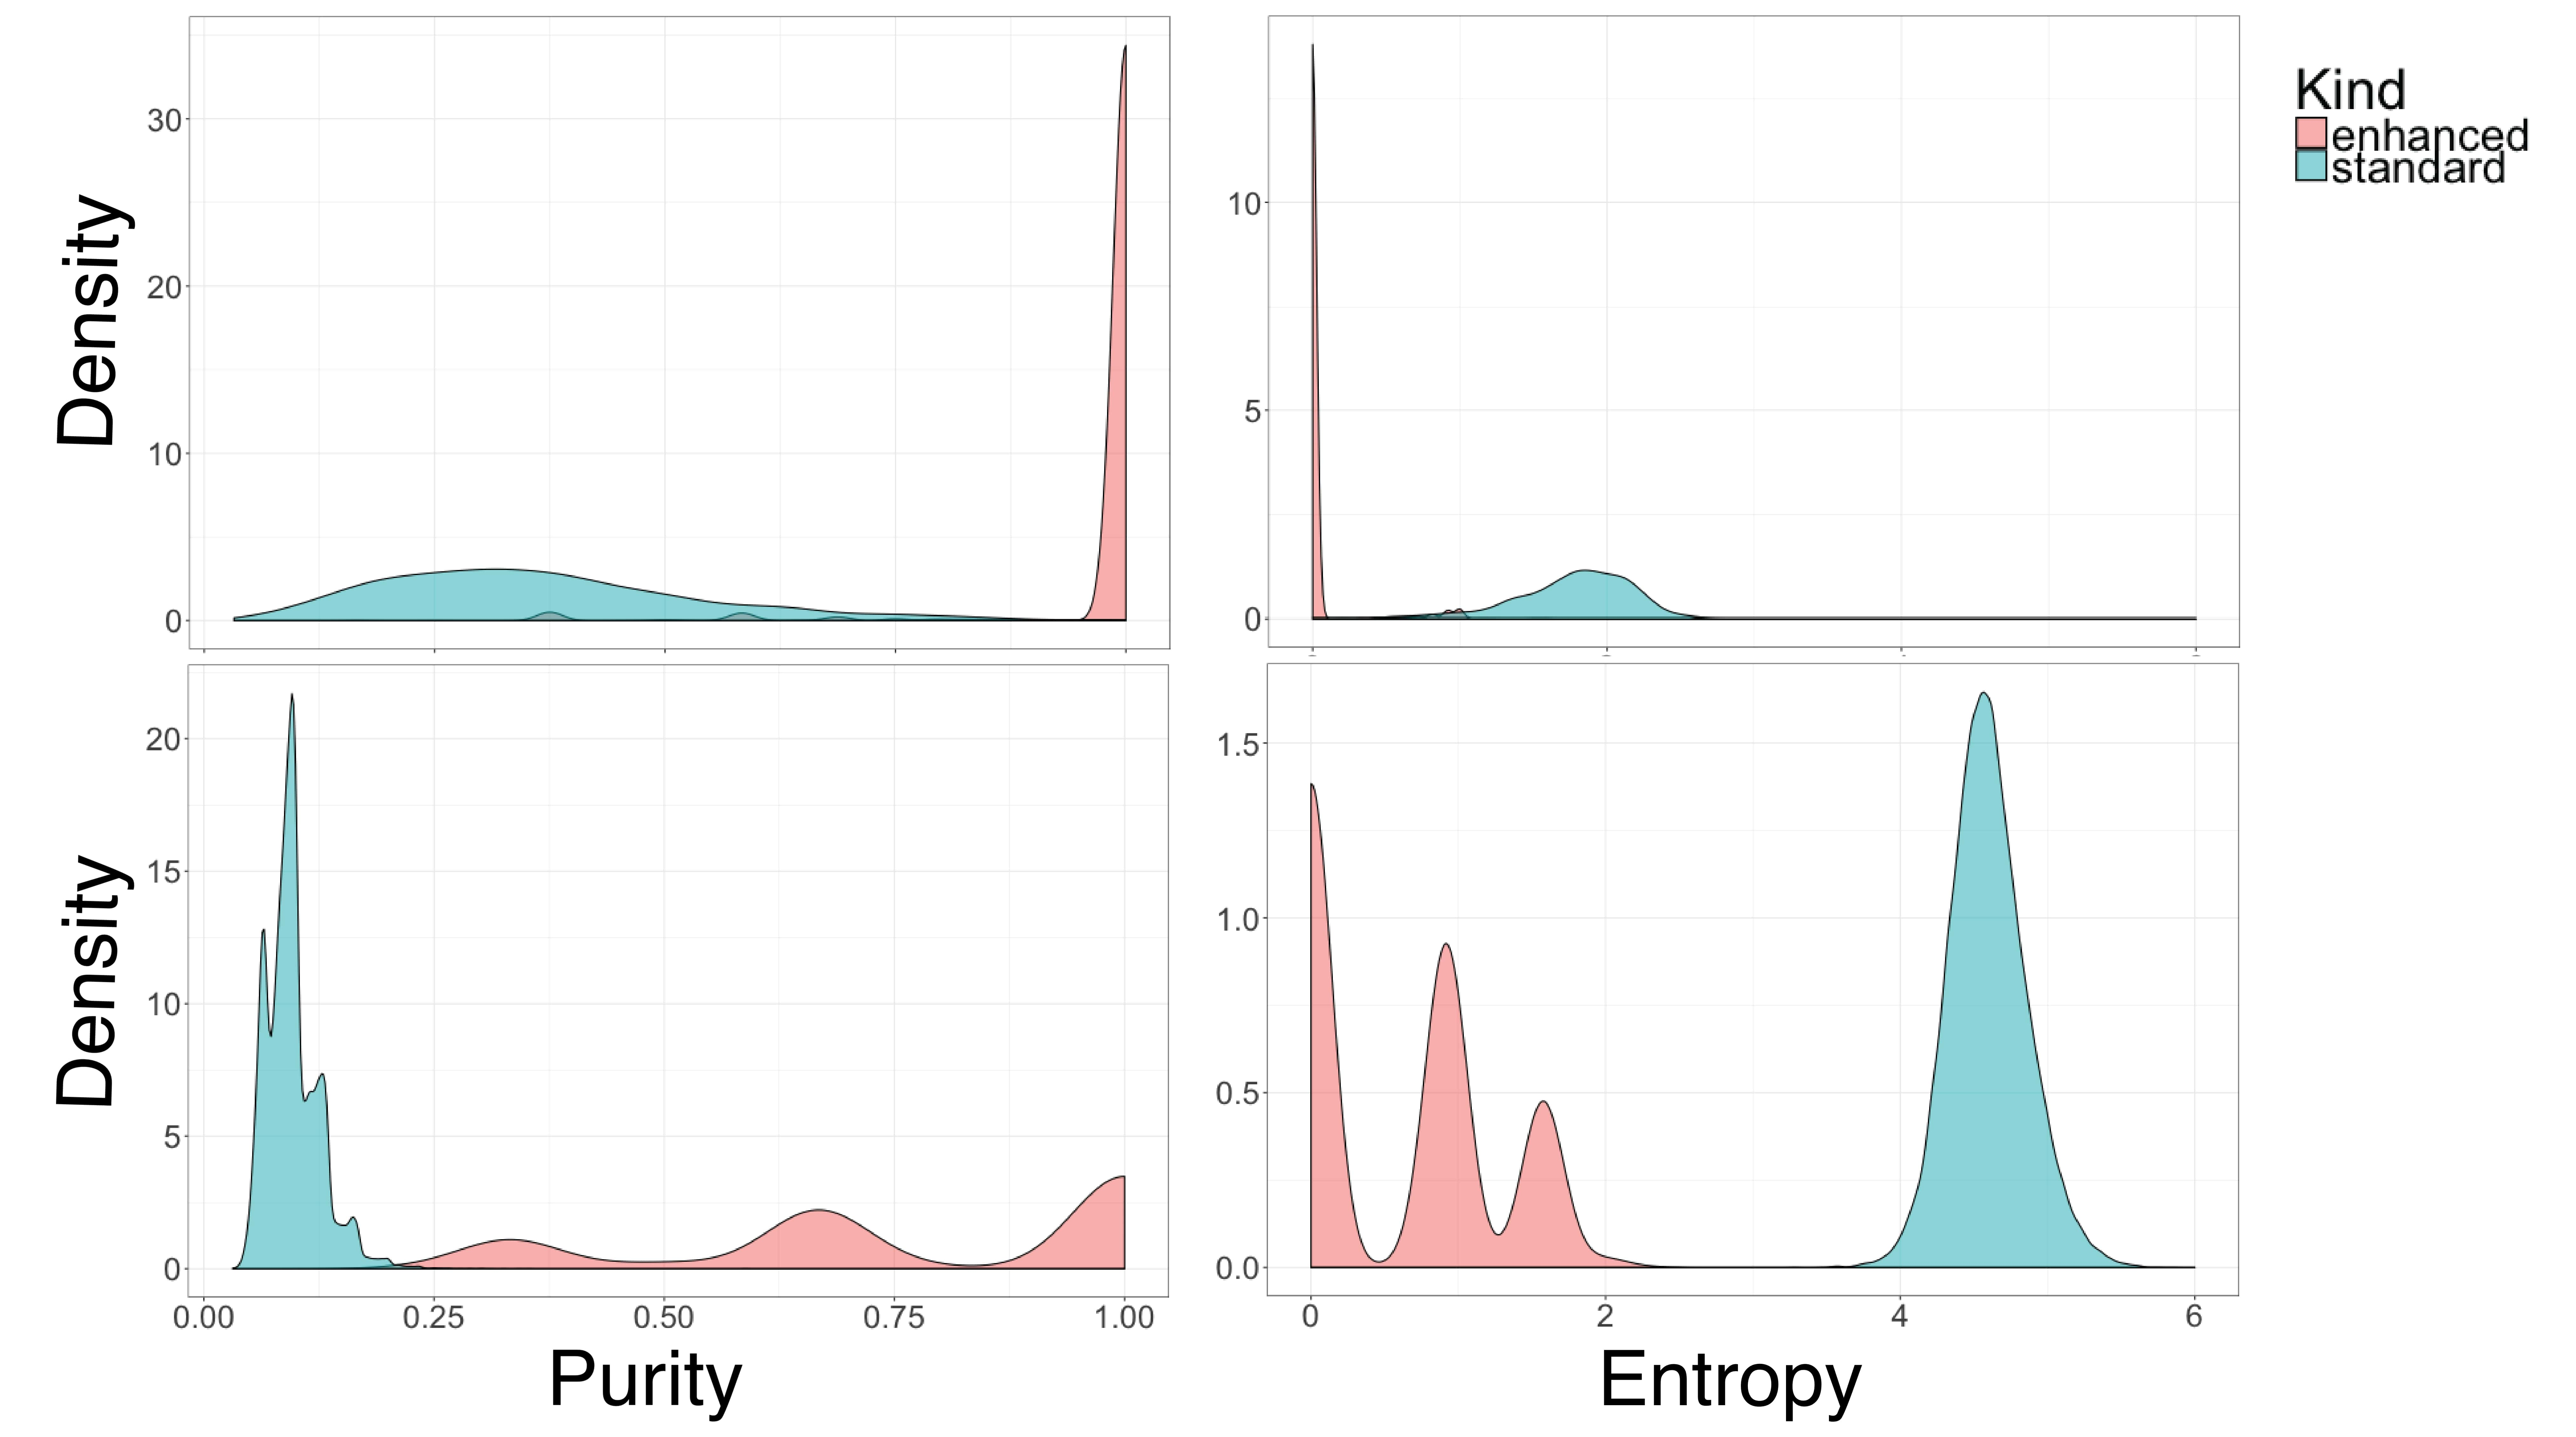
\includegraphics[width=0.95\textwidth]{figures/purity_fig_clean_copy.jpg}
	\vspace{5pt}
	\caption{\small{Clockwise from top left 1) Purity in dataset one for enhanced and 3' barcodes 2) Shannon index in dataset one for enhanced and 3' barcodes 3) Shannon index in dataset two for enhanced and 3' barcodes 4) Purity in dataset two for enhanced and 3' barcodes.}}
    \label{fig:purity}
  \end{center}
  \vspace{-10pt}
 % \vspace{1pt}
\end{figure}

Minerva was able to identify subgroups in Read Clouds that largely corresponded to individual fragments of DNA. We term these subgroups 'Enhanced Read Clouds'. We measured the quality of each enhanced Read Cloud using two metrics: shannon entropy index $H = \sum{p_i\log{p_i}}$ and purity $P = \max(\vec{p})$ where $p_i$ indicates the proportion of an enhanced Read Cloud that belongs to each fragment. These values are shown in figure \ref{fig:purity} as compared to Read Clouds which were not enhanced ('standard' Read Clouds). In general, Minerva produced a large number of perfect ($P=1, H=0$) enhanced Read Clouds.

We also tested whether the quality of the enhanced Read Clouds changed with the number of reads in the Read Cloud. We found a small inverse relationship between Read Cloud size and purity but established that our previous results were not being inflated by a large number of very small enhanced Read Cloud (supplementary figure 2). Note that enhanced Read Clouds of size 1 would be trivially perfect and are always excluded from results. 

In testing we found three parameters that seemed to have the most effect of Minerva's performance. The number of links required between reads to form a cluster ($eps$), the \textit{k}-mer size used to make minimizing \textit{k}-mers ($K$), and the maximum allowed frequency of each read ($maxk$). In supplementary figure 3 we show how these parameters affect Minerva's performance under three different metrics: mean enhanced barcode purity, mean enhanced barcode size, and total reads clustered. Large, pure, and complete clusters being the ideal. We found that Minerva's parameters could be used to tune performance between very large and very pure enhanced barcodes depending on the downstream application.

\subsection*{ Enhanced Read Clouds can be Clustered into Meaningful Groups}
\label{sec:LDA}

After deconvolving barcodes into Enhanced Read Clouds it is useful to group Enhanced Read Clouds that likely came from the same genome. This is essentially a clustering problem. Initially we explored graph based approaches similar to our algorithm for Read Cloud deconvolution. These algorithms relied on the assumption that elements being clustered would have small numbers of distinguishing elements and a relatively high {\it a priori} probability of originating from the same cluster. When dealing with individual barcodes these assumptions proved reasonable; faced with the complexity of a full dataset these assumptions became inaccurate and graph based algorithms performed poorly.

With relatively little structure in the data that could be known {\it a priori} we turned to topic modeling algorithms to discover implicit genetic structures in our data. Latent Dirichlet Allocation is a classic model in Natural Language Processing \citep{Blei2003}. LDA is a generative model that assumes data was created using a certain, well defined, stochastic process. Training the model consists of finding parameters that make it more likely that the observed data would be generated using the given stochastic process; typically this is done with Gibbs sampling.

Typically LDA is used to analyze corpora of natural language. Natural language corpora are organized into documents (e.g. emails or book chapters) that consist of words. The base version of LDA does not consider what order words in a document occur, just how often each word occurs in a given document; this is referred to as a bag-of-words model. Formally, documents are modeled as a sparse vector over a large vocabulary of words where entries represent the number of times a word occurs in the document. LDA maps documents from a high dimensional word-space to a lower dimensional topic-space. In NLP topics typically have intuitive interpretations as thematically consistent units. A key advantage of LDA is that it can distinguish synonyms based on context (i.e. a river bank vs. a financial bank), this may be useful for classifying conserved motifs.

We used LDA to cluster Read Clouds (represented as sets of \textit{k}-mers). Each topic generated by LDA was considered to be a single cluster.

We used LDA to project enhanced and standard Read Clouds into a lower dimensional space. We treated each Read Cloud as a document containing minimum sparse \textit{k}-mers as words. We removed \textit{k}-mers that occured far more often than average in a process similar to removing stop-words in NLP. We ran LDA with hyper-parameter optimization on our Read Cloud-documents and clustered to obtain a topic vector for each Read Cloud using the implementation LDA in Mallet \citep{McCallum2002}. Using X-Means we clustered the topic vectors representing Read Clouds into discrete groups. 

\begin{figure}
  \vspace{-20pt}
  \begin{center}
    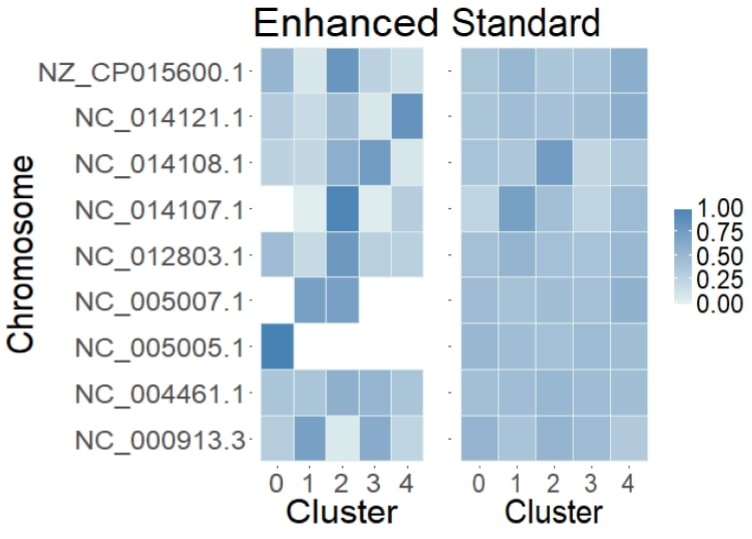
\includegraphics[width=0.65\textwidth]{figures/clusters.jpg}
	\vspace{5pt}
	\caption{\small{Abundance of different chromosomes across clusters as assigned by LDA. Enhanced Read Clouds dramatically improve LDA's ability to distinguish structure in Dataset 1. This figure uses the same deconvolution as figure \ref{fig:purity}}}
    \label{fig:q7}
  \end{center}
  \vspace{-10pt}
 % \vspace{1pt}
\end{figure}

With standard Read Clouds LDA essentially cannot distinguish any structure, with enhanced Read Clouds LDA can generate clusters that are less diverse. The clusterings can be compared in figure \ref{fig:q7}. This could be used to improve assemblies by clustering similar reads and reducing spurious connections. Note that we denote chromosomes rather than genomes in the figure since our process does not attempt to link chromosomes from the same organisms.

\subsection*{ Enhanced Read Clouds Improve Short Read Taxonomic Assignment}
\label{sec:kraken}

We observed that reads from a single linked fragment could be classified using any short read taxonomic classifier. These classifiers, however, often have trade offs between recall and precision. Enhanced Read Clouds can be used to improve recall of a short read classifier without harming precision.

Many of the reads classified by short read taxonomic classifiers cannot be assigned to low taxonomic ranks. However, all reads from the same fragment of DNA must all have the same taxonomic rank. Read Clouds can be used to promote unspecific taxonomic assignments.  Any read with a taxonomic rank that is an antecedent of a lower taxonomic rank in the same Read Cloud can be promoted to the lower rank, provided there are no conflicts with other ranks in the same cloud. Enhanced Read Clouds reduce the risk of conflicting ranks and make it more likely that reads can be promoted.

We used Minerva to improve the specificity of short read taxonomic assignments obtained from Kraken, a popular pseudo-alignment based tool \citep{Wood2014}. We selected Kraken because it was found to have good precision but relatively poor recall in a study by \citep{McIntyre2017}. 

\begin{table}[]
\caption{Taxonomic Promotion. \small{The number of reads which could be promoted using standard or enhanced read clouds in a deconvolution of dataset 1. This figure uses the same deconvolution as figure \ref{fig:purity}. Cases where enhanced read clouds did not outperform standard read clouds are omitted, there are no cases where standard outperformed enhanced.}}
\label{taxapromote}
\begin{tabular}{|l|l|llll|}
\hline
Original Rank           & Promoted Rank          &  Enhanced &  Standard & Difference & Ratio \\
\hline \hline
Bacteria                & {\it Enterobacter cloacae}   &  3        & 2         & 1          &  1.5  \\
Proteobacteria          & {\it Enterobacter cloacae}   &  24       & 17        & 7          &  1.41 \\
Gammaproteobacteria     & {\it Enterobacter cloacae}   &  21       & 13        & 8          &  1.62 \\
Enterobacterales        & {\it Enterobacter cloacae}   &  87       & 72        & 15         &  1.21 \\
Enterobacteriaceae      & {\it Enterobacter cloacae}   &  765      & 642       & 123        &  1.19 \\
\hline
Bacteria                & {\it Escherichia coli}       &  9        & 6         & 3          &  1.5  \\
Proteobacteria          & {\it Escherichia coli}       &  8        & 7         & 1          &  1.14 \\
Enterobacterales        & {\it Escherichia coli}       &  17       & 13        & 4          &  1.31 \\
Enterobacteriaceae      & {\it Escherichia coli}       &  9221     & 7846      & 1375       &  1.18 \\
Escherichia             & {\it Escherichia coli}       &  201      & 198       & 3          &  1.02 \\
\hline
Gammaproteobacteria     & {\it Pseudomonas antarctica} &  3        & 2         & 1          &  1.5  \\
Pseudomonas             & {\it Pseudomonas antarctica} &  256      & 200       & 56         & 1.28  \\
\hline

\end{tabular} 
\end{table}

Using the technique described above we were able to rescue a large number of reads from unspecific taxonomic assignments. We rescued reads using both enhanced Read Clouds and standard Read Clouds. In every case rescue with enhanced Read Clouds matched or outperformed rescue with standard Read Clouds. All cases where rescue with enhanced Read Clouds outperformed standard Read Clouds for Dataset 1 are shown in table \ref{taxapromote}. All observed taxonomic assignments were correct after promotion. Without enhanced barcodes many annotations cannot be rescued or are incorrect.



